\subsection{Emulator}

Emulator is great way to test your codes and get in touch with MARK II without
use of FPGA.

Whole emulator is written in python only. This include SoC too. You can run
MARK II emulator in two modes, in CLI mode and GUI mode.

CLI mode is more simple, you just specify what MIF load into ROM0 and where to
connect UART0 and done. Emulator then start code in ROM0 like real hardware
does. You didn't see any result but you can communicate with CPU using UART and
for example socat with some serial terminal.

GUI mode is great for debugging purposes. GUI is written in tkinter and is
relative simply. But contains all what is needed for debugging. You can step
your program. You can view all memories, all registers, set breakpoint and run
to it. Also you can see disassembled content of memory.

Remember, not whole SoC is emulated. Emulated peripherals are only these what
is important. This mean:

\begin{itemize}
   \item cpu0
   \item rom0 - CPU start execution from here
   \item ram0 - on FPGA this is fastest ram
   \item ram1 - on FPGA this will become external SDRAM soon (at this time is implemented in same way as ram0)
   \item intController - is necessary for CPU
   \item uart0 - we want some way to communicate (work only at 9600 8N1, ignoring all settings)
\end{itemize}

\subsubsection{How one can work with CLI emulator?}

Simply, write your code in .asm file, translate it and link it into loadable
module (.ldm), the use utility ldm2mif and generate mif file for rom0.
Something like this.

\begin{lstlisting}[language=bash, frame=single]
    $ vim main.asm
    $ assembler --skip-linker main.asm
    $ ldm2mif main.ldm
    $ ls
    main.asm main.ldm main.mif
\end{lstlisting}

Now, you have to decide where to bind UART0, lets say, we want virtual serial
port to connect it like when real hardware is connected. Best way to do on
Linux is use socat and pty.

\begin{lstlisting}[language=bash, frame=single]
    $ socat -d -d pty,raw,echo=0 pty,raw,echo=0
    2017/06/02 11:41:50 socat[2252] N PTY is /dev/pts/1
    2017/06/02 11:41:50 socat[2252] N PTY is /dev/pts/2
    2017/06/02 11:41:50 socat[2252] N starting data transfer loop with FDs [5,5] and [7,7]
\end{lstlisting}

As you can see, we get two serial port /dev/pts/1 and /dev/pts/2. They are
connected together with "virtual null modem cable". So, we open can listen on
pts/2 and connect emulator to pts/1. For listening we can use cat.

\begin{lstlisting}[language=bash, frame=single]
    $ cat /dev/pts/2
\end{lstlisting}

And now is time to run your emulator.

\begin{lstlisting}[language=bash, frame=single]
    $ emulator -p /dev/pts/1 -r main.mif
    MARK-II GUI emulator v0.1.9_1
    UART0 mapped into "/dev/pts/1"
    ROM0 loaded with "main.mif"
    For exit from emulator please use CTRL+C.
\end{lstlisting}

That is all. If you want to exit, use CTRL+C.

\subsubsection{How one can work with GUI emulator?}

This is almost same as CLI. So, create your mif in same way.

\begin{lstlisting}[language=bash, frame=single]
    $ vim main.asm
    $ assembler --skip-linker main.asm
    $ ldm2mif main.ldm
    $ ls
    main.asm main.ldm main.mif
\end{lstlisting}

Open pair of serial ports. (note: you can use real port, just give emulator as
parameter something like /dev/ttyUSB0)

\begin{lstlisting}[language=bash, frame=single]
    $ socat -d -d pty,raw,echo=0 pty,raw,echo=0
    2017/06/02 11:41:50 socat[2252] N PTY is /dev/pts/1
    2017/06/02 11:41:50 socat[2252] N PTY is /dev/pts/2
    2017/06/02 11:41:50 socat[2252] N starting data transfer loop with FDs [5,5] and [7,7]
\end{lstlisting}

Listen on the port.

\begin{lstlisting}[language=bash, frame=single]
    $ cat /dev/pts/2
\end{lstlisting}

And run emulator.

\begin{lstlisting}[language=bash, frame=single]
    $ emulator -g -p /dev/pts/1 -r main.mif
    MARK-II GUI emulator v0.1.9_1
    UART0 mapped into "/dev/pts/1"
    ROM0 loaded with "main.mif"
\end{lstlisting}

New window appear, you can see GUI at image \ref{fig:gui_emulator}. Controlling
is simple. Use tick button to execute one instruction, use reset to reset SoC
and exit to exit from emulator. "Run to" can be used for breakpoint. And you
should see memories contents and also registers contents.

\begin{figure}[h]
    \centering
    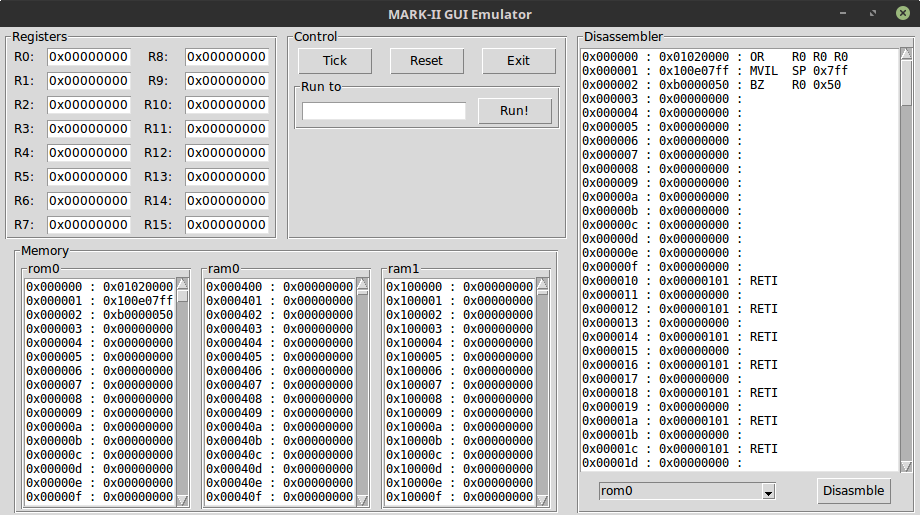
\includegraphics[width=\textwidth]{img/emulator.png}
    \caption{MARK-II GUI Emulator}
    \label{fig:gui_emulator}
\end{figure}
